\section{Methodology}
\label{sec:meth}


\subsection{Beschrijving van de data}
De dataset die gebruikt gaat worden om deze vragen te beantwoorden is een verzameling van troonredes sinds 1814. De gehele dataset bestaat uit 172 verschillende troonredes welke in totaal uit 224165 woorden bestaan, deze set zullen we vanaf nu het corpus noemen. Deze troonredes zijn terug te vinden op www.troonredes.nl~\citep{troonredes} . Om een duidelijker beeld te geven van de troonredes een korte uitleg van wat de troonredes nu precies zijn en waar ze vandaan komen. 

De troonrede wordt nu jaarlijks door de koning(in) uitgesproken op Prinsjesdag, de 3de dinsdag van september. Deze dag is ook de opening van het parlementaire jaar. In de 19de eeuw viel de opening van de Staten-generaal op de eerste maandag van november en later op de 3de maandag van oktober. Voor 1904 werden de troonredes uitgesproken in de vergaderzaal van de 2de kamer. Sinds 1904 worden de troonredes voor de ridderzaal op het binnenhof in Den Haag uitgesproken. De troonrede wordt live uitgezonden op televisie en is na te lezen op de website van de Nederlandse overheid. De eerste troonrede werd in 1814 als een algehele toespraak voor de Staten-generaal gehouden. De troonredes worden vooral gebruikt om wets- en beleidsveranderingen door te geven, als beschouwing op het afgelopen jaar en de staat van het land. In recentere jaren heeft deze beschouwing zich ook uitgebreid naar gebeurtenissen door de hele wereld die invloed uitoefenen op de Nederlandse staat. Ook wordt sinds 1918 het regeerprogramma voor het komende jaar in de troonredes behandelt. Sinds 1848 worden de troonredes geschreven door ministers vanwege een grondwetsherziening waardoor de ministers verantwoordelijk werden voor al het doen en laten van de koning(in). Hiermee werd het kabinet verantwoordelijk voor de uitspraken die gedaan worden in de troonredes.~\citep{overheid} Dit zorgt ervoor dat de troonredes een beeld geven van wat de Nederlandse regering op dat moment belangrijk vindt en zijn ze in die zin een weerspiegeling van de dan heersende politieke urgentie.

Om een duidelijker beeld te geven van de inhoud en omvang van de troonredes geeft tabel \ref{statistieken} een kort overzicht met enkele statistieken. Hierbij is de langste troonrede die van 1993 en de kortste troonrede die van 1880.

\begin{table}[H]
\centering
\begin{tabular}{lrrr}
\toprule
{} &  Paragrafen &  Zinnen &  Woorden \\
\midrule
Gehele corpus &        3887 &   10415 &   224165 \\
Gemiddeld &          22 &      60 &     1303 \\
Langste troonrede &          39 &     191 &     3495 \\
Kortste troonrede &          16 &      20 &      343 \\
\bottomrule
\end{tabular}
\caption{Troonrede statistieken}
\label{statistieken}
\end{table}

De grafiek in figuur \ref{inhoud} geeft een beeld van de grootte van de troonredes over de jaren aan de hand van het aantal zinnen en paragrafen per jaar. Figuur \ref{woorden} toont een grafiek die weergeeft hoeveel woorden de troonrede elk jaar bevatte.

\begin{figure}[H]
\begin{center}
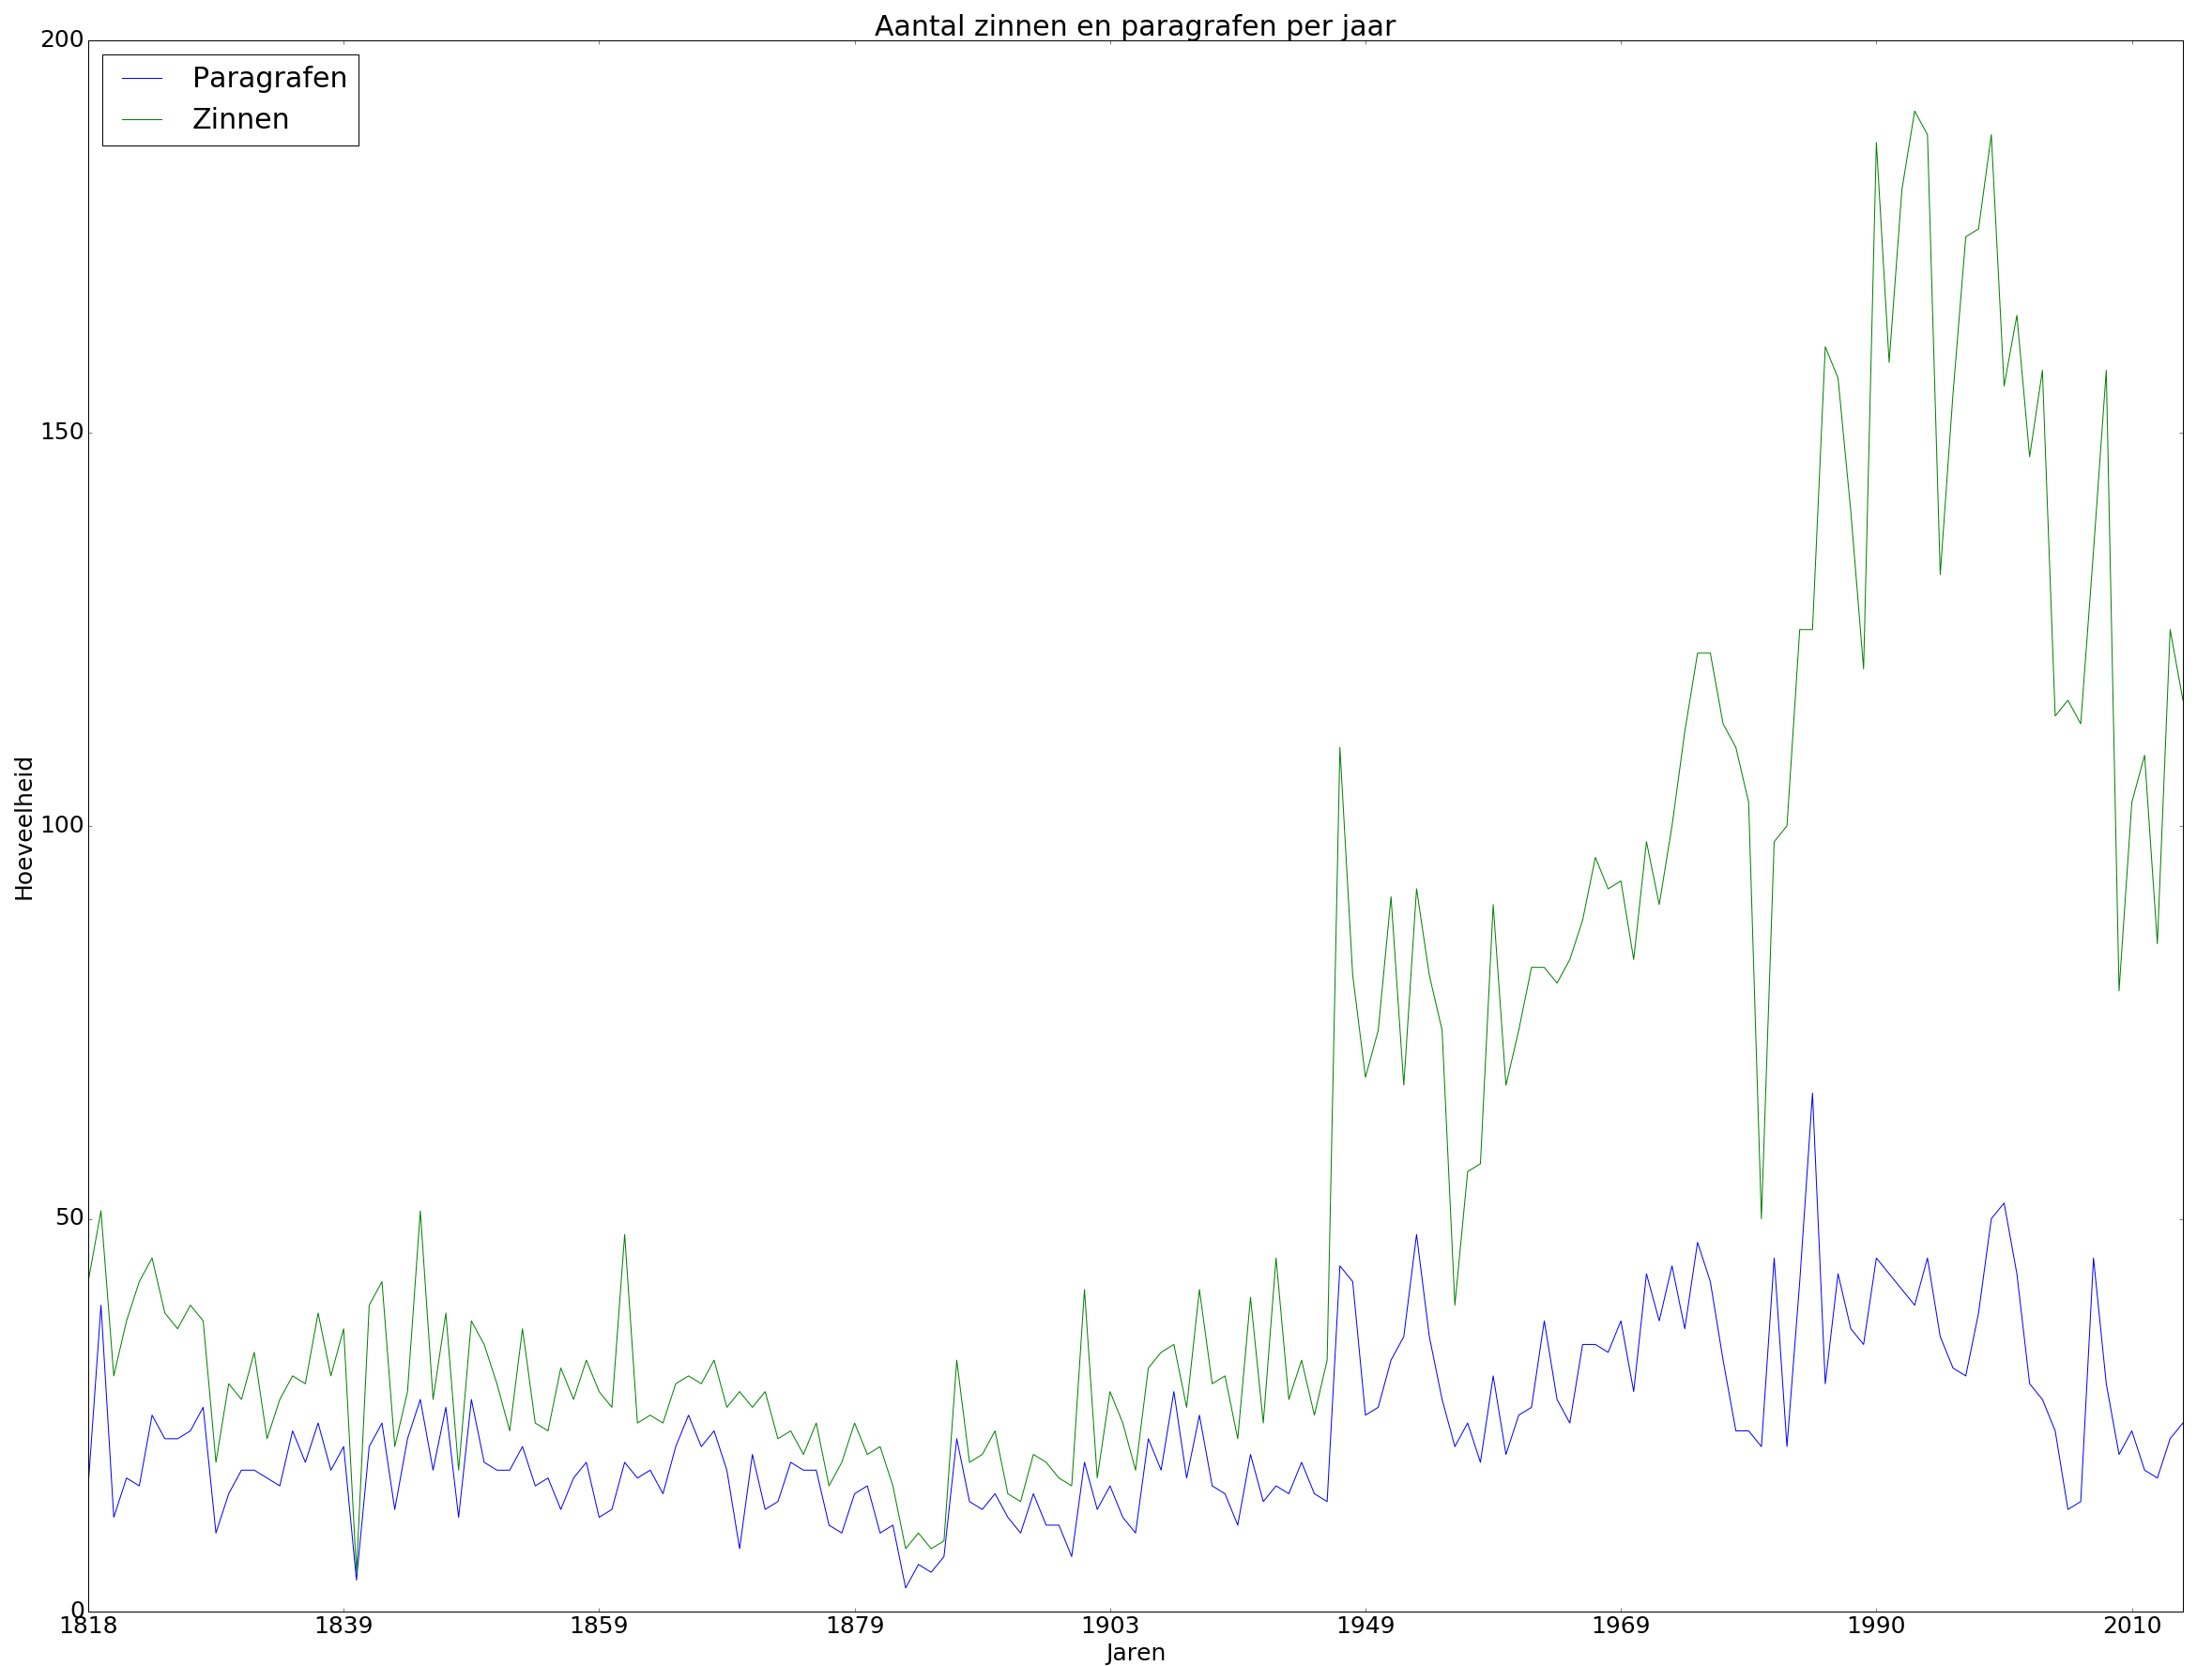
\includegraphics[width=1.2\textwidth]{fig/Inhoudverdeling}
\caption{\label{inhoud} Weergave van het aantal zinnen en paragrafen per jaar.}
\end{center}
\end{figure}

\begin{figure}[H]
\begin{center}
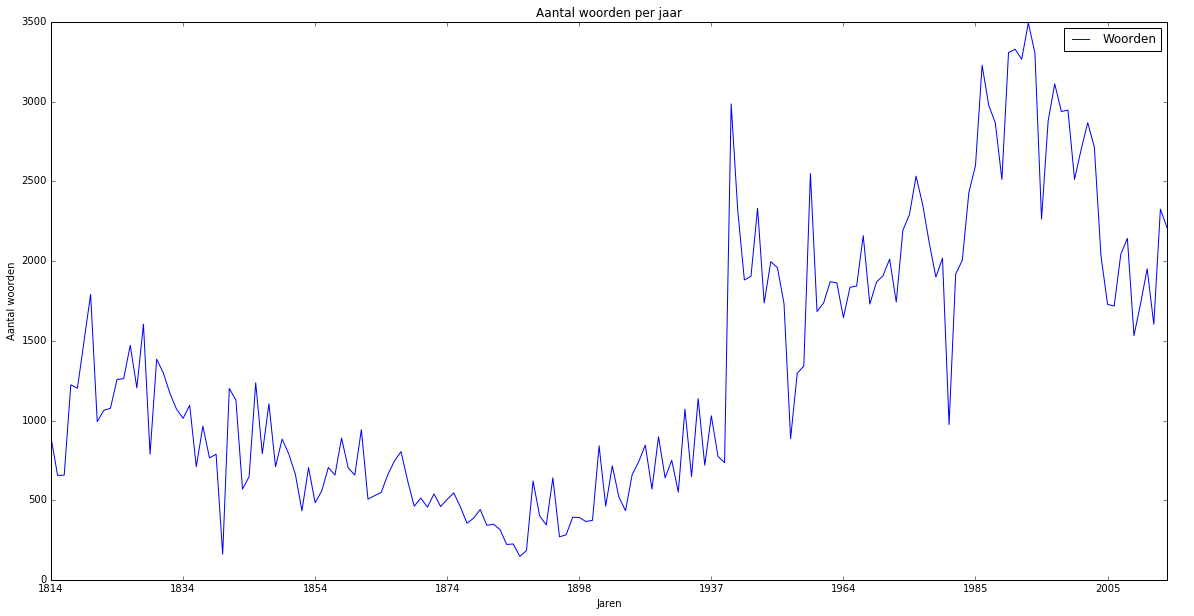
\includegraphics[width=1.2\textwidth]{fig/Woordverdeling}
\caption{\label{woorden} Weergave van het aantal woorden per jaar.}
\end{center}
\end{figure}

Opmerkelijk is hier de stijging in het aantal zinnen en woorden per troonrede na 1937. Deze periode correleert met het einde van de Tweede Wereldoorlog. Hierdoor kan deze verandering in troonrede grootte mogelijk verklaard worden door het feit dat er in die periode terug is gekeken op de oorlog. Dit mogelijk doordat er in die oorlogstijd geen troonredes uitgesproken zijn, hierover verdere informatie in \ref{sssec 1}. Omdat er in die periode geen troonredes uitgesproken zijn had men een grotere periode om op te reflecteren. Ook zal er mogelijk veel aandacht besteed zijn aan het weergeven dat de Nederlandse regering weer kon regeren.

\subsubsection{Missende data} \label{sssec 1}
Er zijn verscheidene jaren waarvan er geen data beschikbaar is, dit doordat er niet elk jaar een troonrede gegeven is. Dit heeft verschillende redenen, zoals oorlogen, angst voor rellen, onvrede over het kabinet of gezondheidsredenen omtrent de koning(in). Dit zorgt ervoor dat niet elk jaar sinds 1814 wordt gerepresenteerd door een troonrede. Omdat de inhoud van de troonredes als verzamelde dataset wordt gebruikt heeft dit minimaal invloed op de uiteindelijke uitkomsten van het onderzoek dat er jaren missen. Door de missende jaren is het weergeven van de verschuiving in onderwerpen mogelijk niet volledig representatief, omdat er geen uitspraken gedaan kunnen worden over de missende jaren.
In tabel \ref{missing} een overzicht van de jaren waar geen troonredes van zijn en de reden dat er in die jaren geen troonrede is gegeven:

\begin{table}[H]
\centering
\begin{tabular}{ll}
\toprule
{} &                       reden \\
Jaren     &                             \\
\midrule
1888-1890 &  Verhindering wegens ziekte van de koning en interne beleidsproblemen\\
\\
1905-1924 &         Eerste wereldoorlog en politieke instabiliteit\\
\\
1940-1947 &         Tweede wereldoorlog en politieke instabiliteit\\
\bottomrule
\end{tabular}
\caption{Missende troonredes}
\label{missing}
\end{table}

\subsubsection{Kwaliteit van de data}
De data waarmee gewerkt zal worden zijn 172 troonredes die in de laatste 200 jaar zijn uitgesproken. Deze troonredes zijn binnengehaald vanaf www.troonredes.nl~\citep{troonredes} en opgeslagen als html pagina's. Alle troonredes die te vinden zijn op www.troonredes.nl die niet digitaal door de overheid werden aangelever zijn handmatig ingevoerd door de beheerders van de website. De troonredes die niet digitaal opgenomen waren zijn overgetypt vanuit het nationaal archief. De troonredes die nu worden uitgesproken worden ook door de Nederlandse overheid online gepubliceerd, waarna deze worden gekopieerd naar de website van www.troonredes.nl.

\subsection{Trefwoord extractie}
Er bestaan verschillende manieren om trefwoorden uit teksten te halen. De meeste eenvoudige manier is door simpelweg te kijken naar de waarschijnlijkheid dat een woord voorkomt. Dit wordt gedaan door te kijken naar de frequentie dat een woord voorkomt in een tekst en dit te delen door het totaal aantal woorden in de tekst. Verder kan men kijken naar een geheel corpus, de meest bekende methode hiervoor is TF-IDF (term frequency–inverse document frequency)\citep{ramos2003using}. Hierbij wordt gekeken naar het voorkomen van woorden in een tekst tegenover het voorkomen in het gehele corpus. De TF-IDF score van een woord is hoog voor een specifieke tekst uit een corpus als deze vaak voorkomt in die tekst, maar verder weinig in de rest van het corpus. Door de frequentie van het voorkomen van een woord in een tekst te compenseren met het voorkomen van het woord in de gehele tekst wordt rekening gehouden met woorden die in het algemeen veel worden gebruikt, zoals stopwoorden \citep{aggarwal2012survey}. 
Daarnaast zijn er methodes gericht op individuele teksten zoals in \cite{matsuo2004keyword}, waar een algoritme gebruikt om trefwoorden uit een enkele tekst te halen zonder gebruik te maken van een corpus. 

\subsection{relevantie van co-occurrences}
Co-occurrences zijn uiteindelijk simpele combinaties van woorden. Deze combinaties geven aan of twee woorden samen voorkomen in een zin, paragraaf of tekst. Hierbij wordt meestal gekeken naar het samen voorkomen in een zin. Met behulp van co-occurrences kan men verschillende clustering methodes uitvoeren. De clusters gevormd door deze methodes kunnen weergeven welke woorden veel invloed hebben op de tekst doordat deze het middelpunt van clusters zullen zijn. Met behulp van deze clusters kunnen de meest belangrijke termen dus worden afgeleid. Ook kunnen met behulp van co-occurrences veel voorkomende multi termen worden gevonden in teksten. Enkele voorbeelden hiervan zijn: "Verenigde Staten" en "Hoger onderwijs". Deze multi termen zijn individuele woorden die ook als één woord gezien kunnen worden. Met behulp van het bepalen van co-occurrences kunnen deze multi termen makkelijk gevonden worden. 

\subsection{co-occurrence extractie}
Men kan op verschillende manieren co-occurrences uit teksten halen. Om deze manieren te verduidelijken gebruiken we de volgende voorbeeldzin: "Het is erg heet". Vanuit deze zin kunnen op de volgende manieren co-occurences worden gehaald. Door enkel co-occurrences te gebruiken van woorden die exact naast elkaar in een zin staan, "Het,is" \& "is,erg" \& "erg,heet". Ook kan het door woorden in een zin volgens de zinsvolgorde met elkaar te koppelen zelfs als er andere woorden tussen, hierdoor zouden "Het,heet" \& "Het,erg" \& "is,heet" ook co-occurrences zijn. Of het kan door alle mogelijke combinaties van woorden in een zin te vormen, dit gebeurt veelal op alfabetische woordvolgorde. Volgens de laatste manier wordt geen rekening meer gehouden met de volgorde van de woorden. De manier die het beste is om de co-occurrences uit de tekst te halen is afhankelijk van wat men uiteindelijk wil kunnen zeggen met de co-occurrences. \citep{shimohata1997retrieving}

\subsection{Invloed van context}
Om een onderwerp of meerdere onderwerpen toe te kunnen wijzen aan een tekst moet men rekening houden met meerdere aspecten. De meest belangrijke hiervan is de context van de tekst. De context bepaald namelijk op welke manier woorden geïnterpreteerd worden en wat ze betekenen voor de tekst. Zo zijn er woorden die enkel voor specifieke domeinen betekenis hebben. Er zijn al meerdere methodes ontwikkeld om rekening te houden met de context van een tekst, maar de meeste hiervan hebben hiervoor een corpus nodig om het context netwerk te kunnen bouwen. Om van een individuele tekst de context te kunnen bepalen kan zeer lastig zijn. Er kan rekening gehouden worden met de context van een corpus door gebruik te maken van woordenboeken voor het specifieke domein dat het corpus bestrijkt. Hiervoor moet men echter wel zelf bepalen wat het domein van het corpus is. \citep{aggarwal2012survey}

\pagebreak
\subsection{Methodes}
Om uit het corpus te kunnen achterhalen of er overkoepelende onderwerpen zijn en wat deze mogelijk zijn wordt er gebruik gemaakt van tekstanalyse technieken. Specifiek wordt er gebruik gemaakt van POS-methodes en co-occurence aanpakken.~\cite{callon1991co}  

Allereerst wordt er met behulp van POS-methodes(Pattern of Speech) gekeken naar het volledige corpus. Deze methodes kijken naar het corpus als geheel en proberen hier patronen uit te halen. Er is specifiek gebruik gemaakt van "Pattern", een Python module, die getraind is voor Nederlandse tekst. Deze module is getraind op verschillende soorten Nederlandse teksten en kan woorden uit de tekst onderverdelen in verschillende categorieën, zoals lidwoorden en zelfstandige naamwoorden. Met behulp van deze module is het corpus gefilterd zodat enkel de zelfstandige naamwoorden zijn overgebleven. De reden dat we enkel zelfstandige naamwoorden gebruiken is het feit dat deze representatief zijn voor de tekst. Dit omdat vanuit de zelfstandige naamwoorden afgeleid kan worden wat het doel en inhoud van de tekst is, want zelfstandige naamwoorden kunnen grammaticaal gezien als het onderwerp van een zin gezien worden. 

Hierna wordt de data van de troonredes gelemmatiseerd. Hierdoor worden de woorden herleid tot hun lemma(stam), waardoor ze kunnen worden geanalyseerd als één term. Enkele voorbeelden hiervan: "steden" wordt herleid tot "stad" en "mensen" kan herleid worden tot "mens". Doordat alle woorden te herleiden tot hun stam wordt er een duidelijk beeld gevormd van alle unieke woorden die gebruikt worden. Hierdoor zal de relatie tussen woorden sneller duidelijk worden, omdat er nu geen onderscheid wordt gemaakt tussen de verschillende vervoegingen van unieke woorden. Met behulp van deze gelemmatiseerde termen wordt een co-occurence matrix opgesteld. Deze matrix wordt aangemaakt door bij te houden hoe vaak een combinatie van 2 termen samen in een paragraaf voorkomen. De matrix geeft uiteindelijk voor alle combinaties van 2 termen de frequentie dat ze samen in een paragraaf voorkomen weer.

Voor alle combinaties uit deze matrix wordt een nabijheidsscore berekend via de volgende definitie: 

 $$S(W_1,W_2)\equiv^{\mathrm{def}\frac{\sum_{c\epsilon W\setminus{W_1,W_2\},PMI(W_1,c)>0}}min(PMI(W_1,c),PMI(W_2,c))}{\sum_{c\epsilon W\{W_1,W_2\},PMI(W_1,c)>0}PMI(W_1,c)}}$$ 

Hierbij is het doel om uit te vinden welke termen relevant zijn en hoe deze zich over tijd met andere termen associëren. De score geeft het verwantschap tussen twee termen "W1" \& "W2" aan. Dit verwantschap wordt bepaald aan de hand van PMI(Pointwise Mutual Information) tussen twee termen \citep{bouma2009normalized}. Hierbij geeft de PMI tussen twee termen "X" \& "Y" aan hoeveel de termen ons over elkaar kunnen vertellen. Hierbij gaat het om het verschil in de kans dat term "X" of "Y" individueel voorkomt in een paragraaf in de tekst en de kans dat termen "X" \& "Y" samen voorkomen in een paragraaf in de tekst. Wiskundig gezien wordt PMI als volgt berekend: 

$$PMI(X,Y)\equiv^{\mathrm{log}\frac{p(X,Y)}{p(X)}}$$

Hierbij is P(X,Y) de kans dat termen "X" \& "Y" samen in een paragraaf voorkomen en P(X) de kans dat term "X" in een paragraaf voorkomt. Dit wordt berekend door het aantal keer dat de term voorkomt in de tekst te delen door het aantal paragrafen. De PMI is een score die positief of negatief kan zijn. Goede collocatie paren van termen hebben een hoge PMI score omdat ze net iets minder samen voorkomen dan dat ze individueel voorkomen.  Een score van 0 betekent dat de termen onafhankelijk van elkaar zijn en er geen uitspraak gedaan kan worden over het voorkomen van term "X" als "Y" voorkomt en vice versa.

Het PMI wordt berekend via de TF(Term Frequency) van een woord. Dit wil zeggen dat er gekeken wordt naar het aantal keren dat het woord voorkomt in de tekst. Als het woord "minister" bijvoorbeeld 5 keer voorkomt in een troonrede heeft het een TF van 5 voor die troonrede. Op deze manier wordt ook de TF voor alle woorden berekend over het gehele corpus. Hierbij worden alle troonredes als één enkele tekst gezien om te bepalen hoe vaak een woord in het gehele corpus voorkomt. Dit wordt gebruikt om de P(X) als volgt te berekenen:

$$P(X)\equiv^{\frac{TF(X)}{Aantal Paragrafen}}$$

Hierbij is de TF(X) de Term Frequency van het woord in het gehele corpus en "Aantal Paragrafen" het aantal paragrafen in het gehele corpus.

De co-occurence matrix wordt gebruikt bij het berekenen van P(X,Y). In de co-occurence matrix wordt bijgehouden hoe vaak twee termen samen in een zin voorkomen. In essentie is dit de TF van de combinatie van termen. Hiermee wordt P(X,Y) op dezelfde manier berekend als P(X), waarbij de TF(X) wordt vervangen door de TF van de co-occurence combinatie vanuit de co-occurence matrix.

De vergelijking voor de nabijheidsscore maakt gebruikt van de termen uit het gehele corpus om context te bepalen. Hiervoor wordt voor elke combinatie termen (W1,W2) gekeken naar de woorden waarmee ze samen in een paragraaf voorkomen. De som van PMI(W,C) voor alle termen (C) uit het corpus waarvoor geldt dat PMI(W,C) \textgreater 0 wordt voor beide termen berekend. Dit betekent dus dat er enkel wordt gekeken naar combinaties van termen die onafhankelijk van elkaar zijn, met een score van 0, of  positief. Als hieruit volgt dat PMI(W1,C) gelijk is aan PMI(W2,C) kan men stellen dat als W1 in een paragraaf voorkomt W2 ook voorkomt en vice versa. Een nabijheidsscore van 0 geeft aan dat de woorden nooit samen in een paragraaf voorkomen. Aan de hand van deze score wordt een gewogen semantisch netwerk gevormd met de termen als nodes en de gewichten op de edges. 

Om de termen binnen dit netwerk te kunnen analyseren wordt gebruik gemaakt van een community detectie algoritme. Het specifieke algoritme dat gebruikt wordt is dat van~\cite{blondel2008fast}. Het doel van dit algoritme is om vanuit het gewogen netwerk clusters te vormen van samenhangende subsets van termen. Om ervoor te zorgen dat enkel de meest relevante termen worden meegegeven aan het community detectie algoritme is een drempelwaarde bepaald. Deze drempelwaarde geeft aan vanaf welke waarde voor de nabijheidsscore de co-occurence combinaties door het algoritme verwerkt worden. De drempelwaarde ligt tussen de 0 en 1 en wordt bepaald door vanaf 0 de score op te hogen. Dit is een handmatig proces waarbij de drempelwaarde is bereikt als er binnen het netwerk een component van meer dan twee nodes verdwijnt. Hiermee worden de zwak verbonden nodes uit het netwerk verwijderd. De drempelwaarde die gevonden is voor ons netwerk is θ=0.65. Het resulterende netwerk is door het community detectie algoritme verwerkt om de verschillende subsets te kunnen identificeren. Vanuit deze subsets zijn onderwerpen bepaald aan de hand van de termen die er onder vallen. Afhankelijk van de termen binnen deze clusters kunnen deze clusters gezien worden als indicatief voor onderwerpen/thema's binnen het corpus. Dit induceren van onderwerpen moet een overzicht geven van de verschillende termen die tot een onderwerp behoren en hoe sterk de samenhang is tussen termen binnen een onderwerp. Ook zou het een beeld moeten geven van de samenhang tussen verschillende onderwerpen. 
